\chapter{Texturing System and Procedural Synthesis}
\label{chap:texturing}

\section{Procedural Texture Generation Architecture}
To achieve complete self-containment without dependency on external image downloads, \textit{Matsuri Nights} implements an autonomous procedural texture synthesizer within \texttt{src/TextureGenerator.h}. At engine startup, if static BMP files are missing from \texttt{assets/textures/}, the generator programmatically synthesizes eight 24-bit uncompressed BMP textures ($256 \times 256$ pixels, exactly 196,662 bytes each).

\subsection{Raw 24-Bit BMP Image Exporter}
The function \texttt{TextureGenerator::writeBMP24} constructs standard Windows BMP files by assembling the 14-byte \texttt{BITMAPFILEHEADER} and 40-byte \texttt{BITMAPINFOHEADER}:
\begin{equation}
\text{RowBytes} = \operatorname{ceil}\left( \frac{\text{width} \times 3}{4} \right) \times 4 = (256 \times 3 + 3) \ \& \ (\sim 3) = 768\,\text{bytes}
\end{equation}
Pixels are transformed from standard RGB into the BGR byte layout expected by the BMP format, handling 4-byte row alignment padding.

\section{The Eight Procedural Texture Synthesizers}
Table~\ref{tab:procedural_textures} summarizes the procedural generation algorithms for the eight scene materials.

\begin{table}[H]
\centering
\small
\begin{tabularx}{\textwidth}{p{3.0cm} p{4.2cm} p{7.0cm}}
\toprule
\textbf{Texture Name} & \textbf{Mapped Geometry} & \textbf{Mathematical Synthesis Algorithm} \\
\midrule
\textbf{Wood Timber} \newline (\texttt{wood\_timber.bmp}) &
Machiya timber framing, Torii crossbeams, stall counters &
Combines longitudinal high-frequency sine waves with multi-octave pseudo-noise to model authentic wood grain fibers and ring density variations. \\
\addlinespace
\textbf{Roof Tiles} \newline (\texttt{roof\_tiles.bmp}) &
Machiya primary \& eave roofs, stall canopies &
Models traditional curved Japanese ceramic tiles (\textit{Kawara}) using periodic vertical cylindrical profile shading overlaid with horizontal tile overlapping lips. \\
\addlinespace
\textbf{Stone Pavement} \newline (\texttt{stone\_pavement.bmp}) &
Ground street pavement, building curbstones &
Generates staggered rectangular granite cobblestones with deep mortar grooves, perturbed with surface roughness noise. \\
\addlinespace
\textbf{Lantern Paper} \newline (\texttt{lantern\_paper.bmp}) &
Chochin paper lanterns, Andon floor lamps &
Simulates translucent handmade mulberry paper (\textit{Washi}) with horizontal bamboo rib line banding and subtle fiber density variations. \\
\addlinespace
\textbf{Tatami Cloth} \newline (\texttt{tatami\_cloth.bmp}) &
Machiya interior ground and upper floor decks &
Models woven rush grass Tatami mat weave patterns with dark fabric border binding bands along mat edges. \\
\addlinespace
\textbf{Gold Leaf} \newline (\texttt{gold\_leaf.bmp}) &
Vanishing illusion box, Torii plaque inscription &
High-frequency metallic noise producing glittering specular micro-facets of hammered decorative gold leaf. \\
\addlinespace
\textbf{Sakura Bark} \newline (\texttt{sakura\_bark.bmp}) &
Cherry blossom tree trunk and main boughs &
Deep charcoal-brown base color perturbed by characteristic horizontal lenticel breathing pores and furrowed bark cracks. \\
\addlinespace
\textbf{Takoyaki Batter} \newline (\texttt{takoyaki\_food.bmp}) &
Hopping takoyaki octopus food balls &
Golden-brown fried batter gradient decorated with green seaweed flakes (\textit{Aonori}) and dark brown Worcestershire sauce drizzle stripes. \\
\bottomrule
\end{tabularx}
\caption{Catalog of Procedural 24-bit BMP Textures (\texttt{src/TextureGenerator.h}).}
\label{tab:procedural_textures}
\end{table}

\section{Texture Mapping and GPU Sampling Pipeline}
Textures are managed via the \texttt{Texture} class (\texttt{src/Texture.h}):
\begin{itemize}
    \item \textbf{Filtering Modes:} Minification uses \texttt{GL\_LINEAR\_MIPMAP\_LINEAR} (trilinear filtering with mipmaps); magnification uses \texttt{GL\_LINEAR}.
    \item \textbf{Wrap Modes:} S and T coordinates are configured to \texttt{GL\_REPEAT}, allowing arbitrary texture repetition across large surface areas (such as the 80m stone street).
    \item \textbf{Texture Tiling:} Each \texttt{SceneNode} maintains a \texttt{textureTiling} uniform scalar, scaling coordinates ($u' = u \cdot \text{tiling}, v' = v \cdot \text{tiling}$) in the fragment shader.
\end{itemize}

\section{Visual Comparison: Textures Enabled vs. Disabled}
Pressing the \textbf{X} key toggles diffuse texture maps globally, revealing the raw underlying material colors and geometric meshes.

\begin{figure}[H]
\centering
\begin{subfigure}[b]{0.48\textwidth}
  \centering
  \IfFileExists{figures/ss_14_textures_disabled.png}{%
    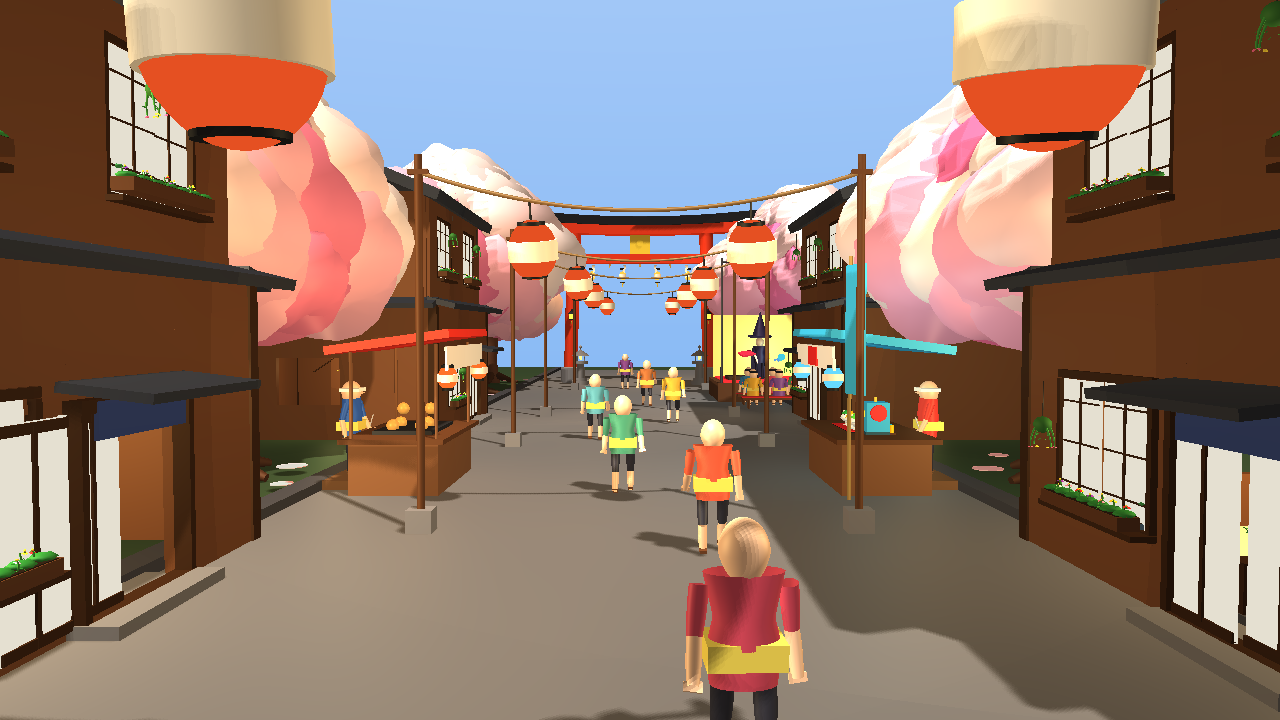
\includegraphics[width=\textwidth]{figures/ss_14_textures_disabled.png}%
  }{\fbox{ss\_14}}
  \caption{Textures Disabled (Raw geometric material colors)}
  \label{fig:tex_off}
\end{subfigure}\hfill
\begin{subfigure}[b]{0.48\textwidth}
  \centering
  \IfFileExists{figures/ss_01_overview_day.png}{%
    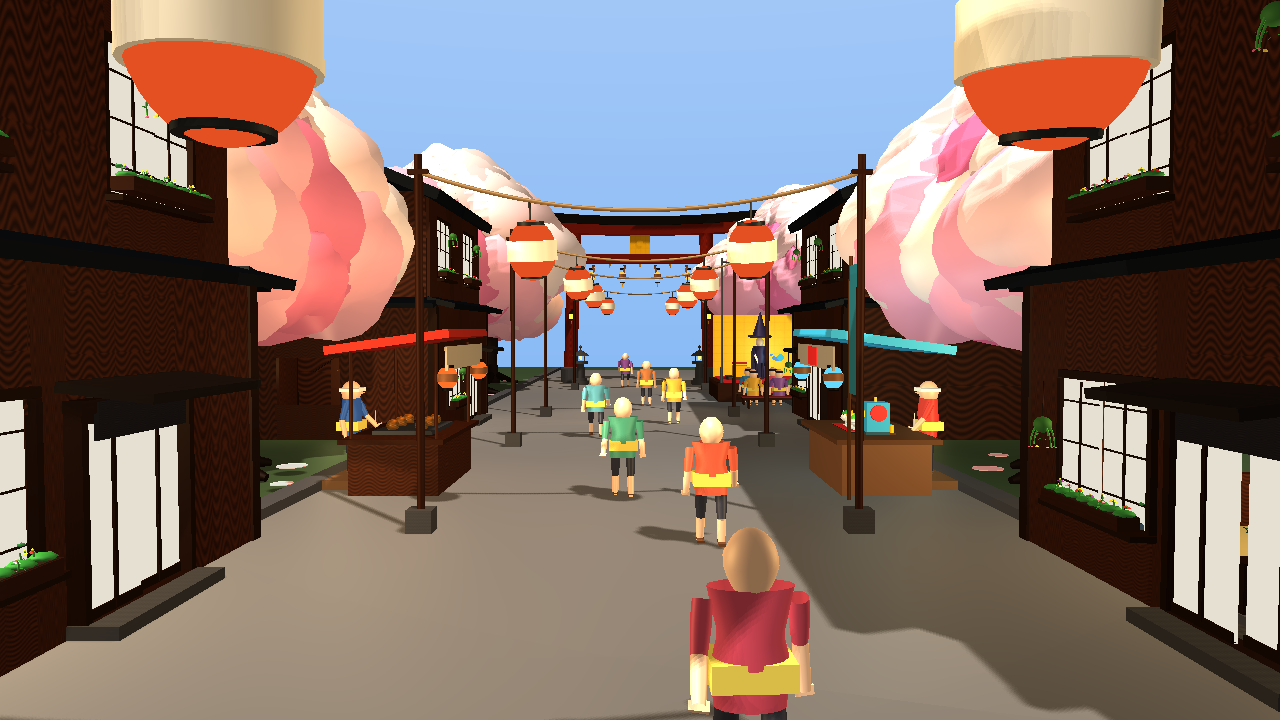
\includegraphics[width=\textwidth]{figures/ss_01_overview_day.png}%
  }{\fbox{ss\_01}}
  \caption{Textures Enabled (Diffuse maps active)}
  \label{fig:tex_on}
\end{subfigure}
\caption{Visual impact of diffuse texture mapping accessible via Key X.}
\label{fig:textures_comparison}
\end{figure}
